\documentclass[wide,a4paper,titlepage,12pt]{mwart}
\usepackage{polski,graphicx,pdflscape}
\usepackage[utf8]{inputenc}
\usepackage{listings}


\title{Dyskretna Transformata Fouriera}
\author{Tymon Tobolski (181037)\\ Jacek Wieczorek (181043)}

% Title page layout (fold)
\makeatletter
\renewcommand{\maketitle}{
\begin{titlepage}
  \begin{center}
    \vspace*{3cm}
    \LARGE \@title \par
    \vspace{2cm}
    \textit{\small Autor:}\par
    \normalsize \@author\par \normalsize
    \vspace{3cm}
    \textit{\small Prowadzący:}\par
    Dr inż. Paweł Biernacki \par
    \vspace{2cm}
    Wydział Elektroniki\\ II rok\\ WT/TN 13:15--15:00 \par
    \vspace{5cm}
    \small \@date
  \end{center}
\end{titlepage}
}
\makeatother
% Title page layout (end)

\begin{document}
  \maketitle
  \section{Cel ćwiczenia} % (fold)
  \label{sec:Cel}
    Celem ćwiczenia jest analiza i porównanie widma różnych sygnałów oraz zbadanie parametrów widma sygnału rzeczywistego i zespolonego.
    
  \section{Algorytm przetwarzający}
    Wykorzystane funkcje:
    \newline
    \begin{itemize}
      \item generujące sygnał (\textbf{sin}, \textbf{cos}, \textbf{prostokat})
			\item wyznaczająca widmo (\textbf{fft})
			\item wyznaczająca parametry widma (\textbf{real}, \textbf{imag}, \textbf{abs})
			\item wyznaczające wykres fazowy (\textbf{angle}, \textbf{unwrap})
			\item generująca sygnał zespolony (\textbf{complex})
    \end{itemize}
  
  \lstset{ %
    language=Octave,                % choose the language of the code
    basicstyle=\scriptsize,       % the size of the fonts that are used for the code
    numbers=left,                   % where to put the line-numbers
    numberstyle=\scriptsize,      % the size of the fonts that are used for the line-numbers
    stepnumber=10,                   % the step between two line-numbers. If it's 1 each line 
                                    % will be numbered
    numbersep=9pt,                  % how far the line-numbers are from the code
    % backgroundcolor=\color{white},  % choose the background color. You must add \usepackage{color}
    showspaces=false,               % show spaces adding particular underscores
    showstringspaces=false,         % underline spaces within strings
    showtabs=false,                 % show tabs within strings adding particular underscores
    % frame=single,                 % adds a frame around the code
    % tabsize=2,                  % sets default tabsize to 2 spaces
    % captionpos=b,                   % sets the caption-position to bottom
    breaklines=true,                % sets automatic line breaking
    % breakatwhitespace=false,        % sets if automatic breaks should only happen at whitespace
    % title=\lstname,                 % show the filename of files included with \lstinputlisting;
                                    % also try caption instead of title
    % escapeinside={\%*}{*)},         % if you want to add a comment within your code
    % morekeywords={*,...}            % if you want to add more keywords to the set
    }
    \lstinputlisting{lab4.m}
    
  % section Wstęp (end)
  
  \section{Analiza widma sygnału sinusoidalnego, który w $N$ próbkach zawiera całkowitą i niecałkowitą liczbę okresów}
		Widmo sygnału sinusoidalnego zawierające w $N$ próbkach niecałowitą liczbę okresów, różni się od widma sygnału o całkowitej liczbie okresów. Dzieje się to dlatego, że dla sygnału o niecałkowitej liczbie okresów zachodzi zjawisko nazywane przeciekiem widma. Występuje ono wtedy, gdy sygnał wejściowy posiada częstotliwość, która nie jest dokładnie równa częstotliwości, dla której wyznaczony jest prążek Dyskretnej Transformaty Fouriera.
		
		Wykresy znajdują się na stronie \pageref{fig1}.

  \section{Próbkowanie i analiza widma sygnału ciągłego}
		{$f_{sin} \in m*fpr/N, m \in {0,1,..,N-1}$} oraz {$f_{sin} \notin m*fpr/N$}
		
		Zgodnie ze wzorem $f(m) = \frac{m*f_{pr}}{N}$ podstawiając odpowiednie wartości $m$ i analizując widma takowych sygnałów zauważamy, że również zachodzi zjawisko przecieków widma, z takich samych powodów jak w pkt 3.
		
		Wykresy znajdują się na stronie \pageref{fig2}.
		
	\section{Analiza widm sygnału sinusoidalnego i prostokątnego}
		\subsection{Sygnał sinusoidalny}
		Wartość rzeczywista widma sygnału sinusoidalnego jest znacznie mniejsza od widma urojonego. Kształtem przypomina natomiast wykres modułu widma sygnału. Wykres modułu widma sygnału, co do wartości jest sumą modułów wartości rzeczywistej i urojonej. Wykres widma amplitudowego (wykres modułu) pokazuje, jakie są amplitudy składowych widmowych sygnału o różnych częstotliwościach. Widmo fazowe ma kształt sygnału piłokształtnego i pokazuje nam jakie składowe fazowe wchodzą w skład sygnału oryginalnego.
		
		Wykresy znajdują się na stronie \pageref{fig3}.
		
		\subsection{Sygnał prostokątny}
		Wykres widma sygnału prostokątnego, w przeciwieństwie do widma sygnału sinusoidalnego, różni się od swojego widma modułu. Wykres urojonej części widma sygnału prostokątnego jest odwrócony względem osi x w stusunku do widma urojonego sygnału sinusoidalnego. Wykres widma fazowego stanowi funkcję liniową.
		
		Wykresy znajdują się na stronie \pageref{fig4}.
		
	\section{Analiza wykresów fazowych sygnałów sinus i cosinus}
		Wykres widma obrazuje zmianę częstotliwości sygnałów sinusoidalnego i cosinusoidalnego. Miejsca wystąpienia skoków pokazuja nam wartości częstotliwości sygnałów. Wykres widma fazowego sygnału cosinusodalnego ma dwa razy wiecej skoków, niż wykres widma fazowego sygnału sinusoidalnego. Wykresy są przesunięte względem siebie o $\frac{\pi}{2}$, czyli różnica faz między sinusem i cosinusem.
	
		Wykresy znajdują się na stronie \pageref{fig5}.
		
	\section{Analiza widma sygnału zespolonego}
		Sygnał zespolony: $x(m) = sin(m) + i*cos(m)$
		
		Wartość rzeczywista widma sygnału zespolonego jest mniejsza od widma urojonego. Różnica jest jednak dużo mniejsza niż w przypadku sygnału rzeczywistego z pkt 5.1. Widmo fazowe, podobnie jak w przypadku sinusoidalnego sygnału rzeczywistego, ma kształt sygnału piłokształtnego. 
		
		
		Wykresy znajdują się na stronach \pageref{fig6} i \pageref{fig7}.

		
	\begin{landscape}
	  \begin{figure}[htbp]
	    \begin{center}
	      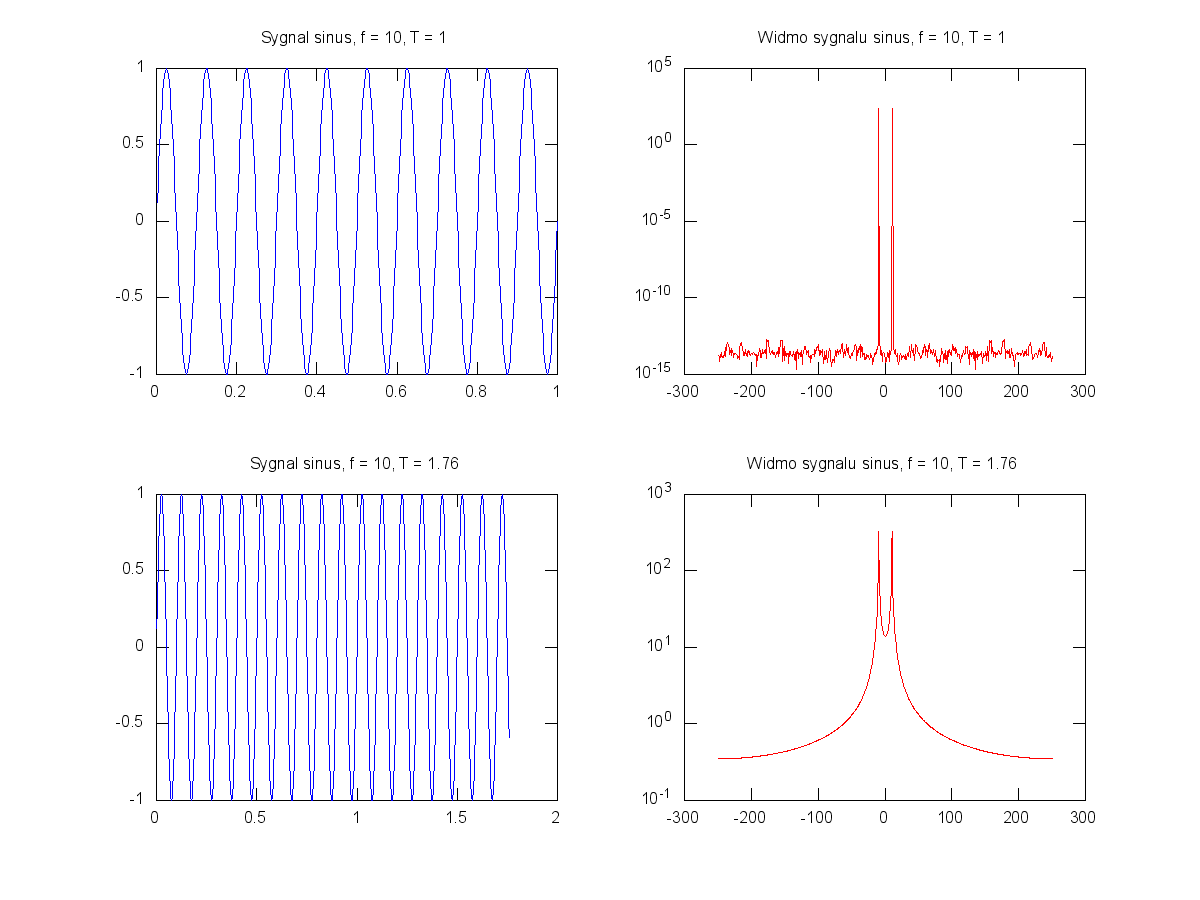
\includegraphics[scale=.5]{out/fig1.png}
	      \caption{\label{fig1} Widmo sygnału sinus}
	    \end{center}
	  \end{figure}
	\end{landscape}
	
	\begin{landscape}
	  \begin{figure}[htbp]
	    \begin{center}
	      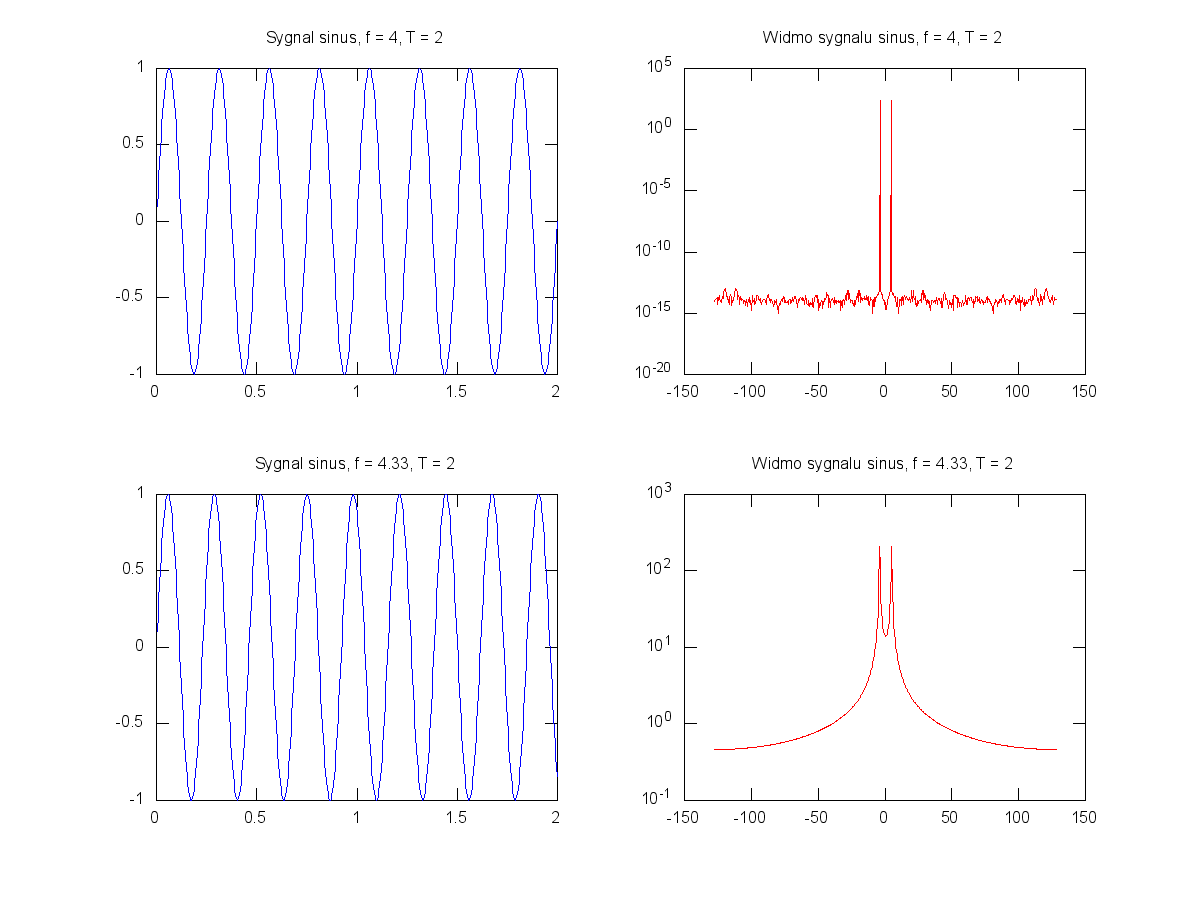
\includegraphics[scale=.5]{out/fig2.png}
	      \caption{\label{fig2} Widmo sygnału sinus}
	    \end{center}
	  \end{figure}
	\end{landscape}
	
	\begin{landscape}
	  \begin{figure}[htbp]
	    \begin{center}
	      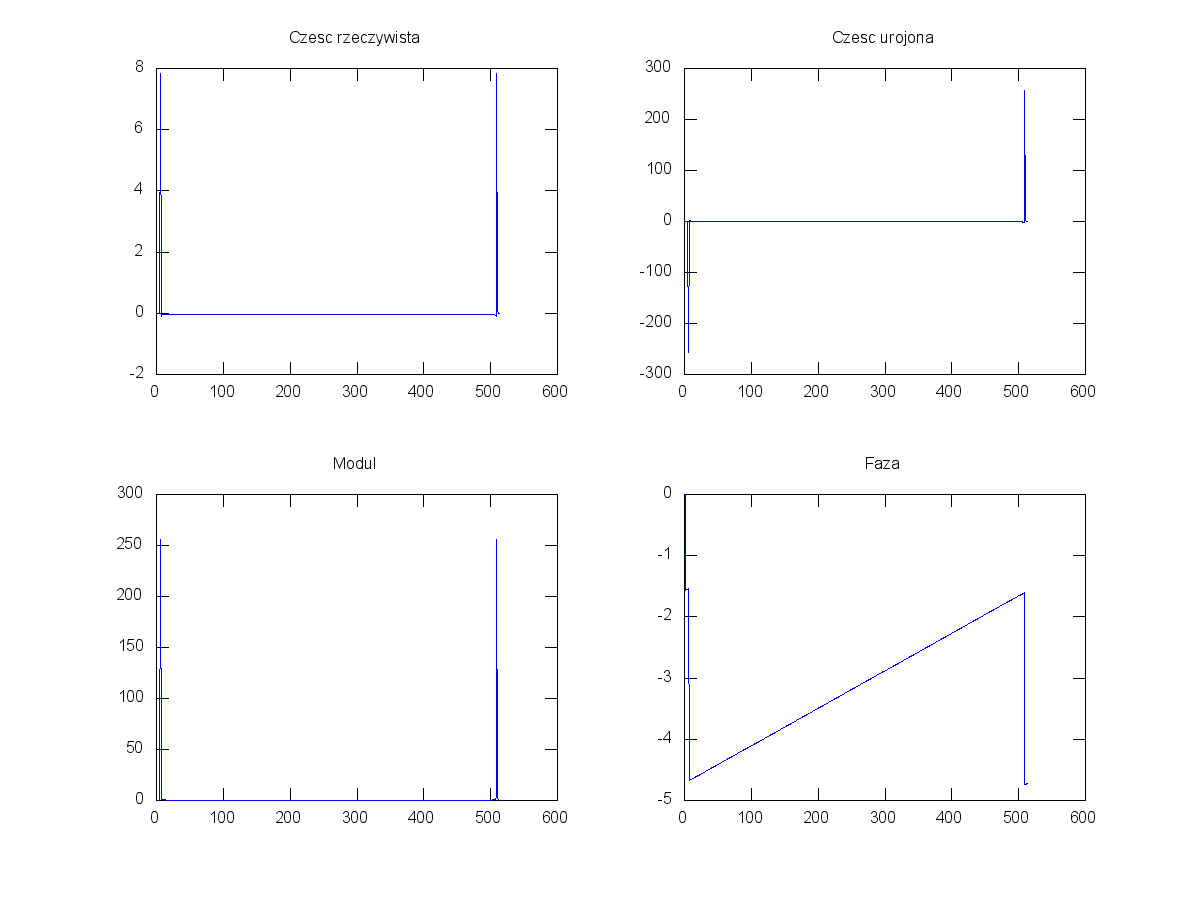
\includegraphics[scale=.5]{out/fig3.png}
	      \caption{\label{fig3} Widmo sygnału sinus}
	    \end{center}
	  \end{figure}
	\end{landscape}
	
	\begin{landscape}
	  \begin{figure}[htbp]
	    \begin{center}
	      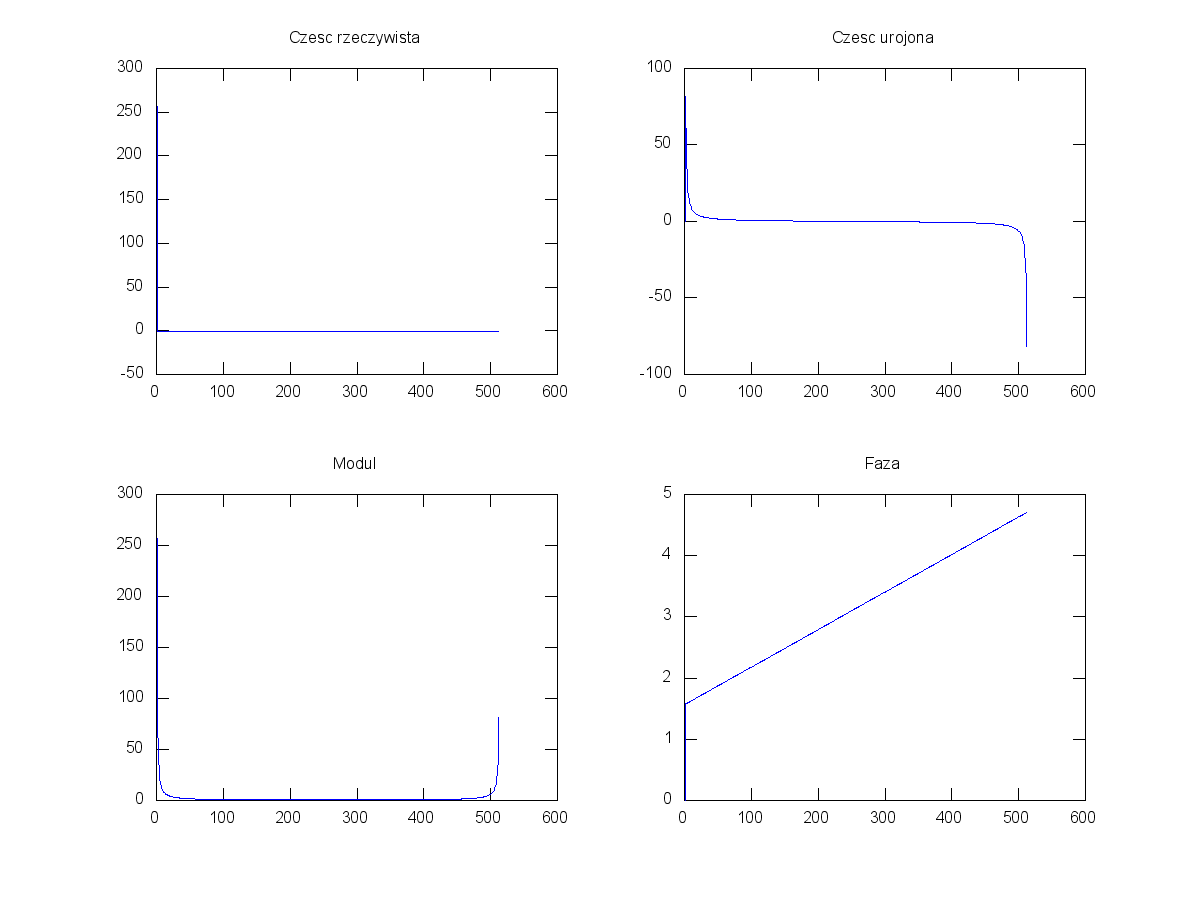
\includegraphics[scale=.5]{out/fig4.png}
	      \caption{\label{fig4} Widmo sygnału prostokątnego}
	    \end{center}
	  \end{figure}
	\end{landscape}
	
	\begin{landscape}
	  \begin{figure}[htbp]
	    \begin{center}
	      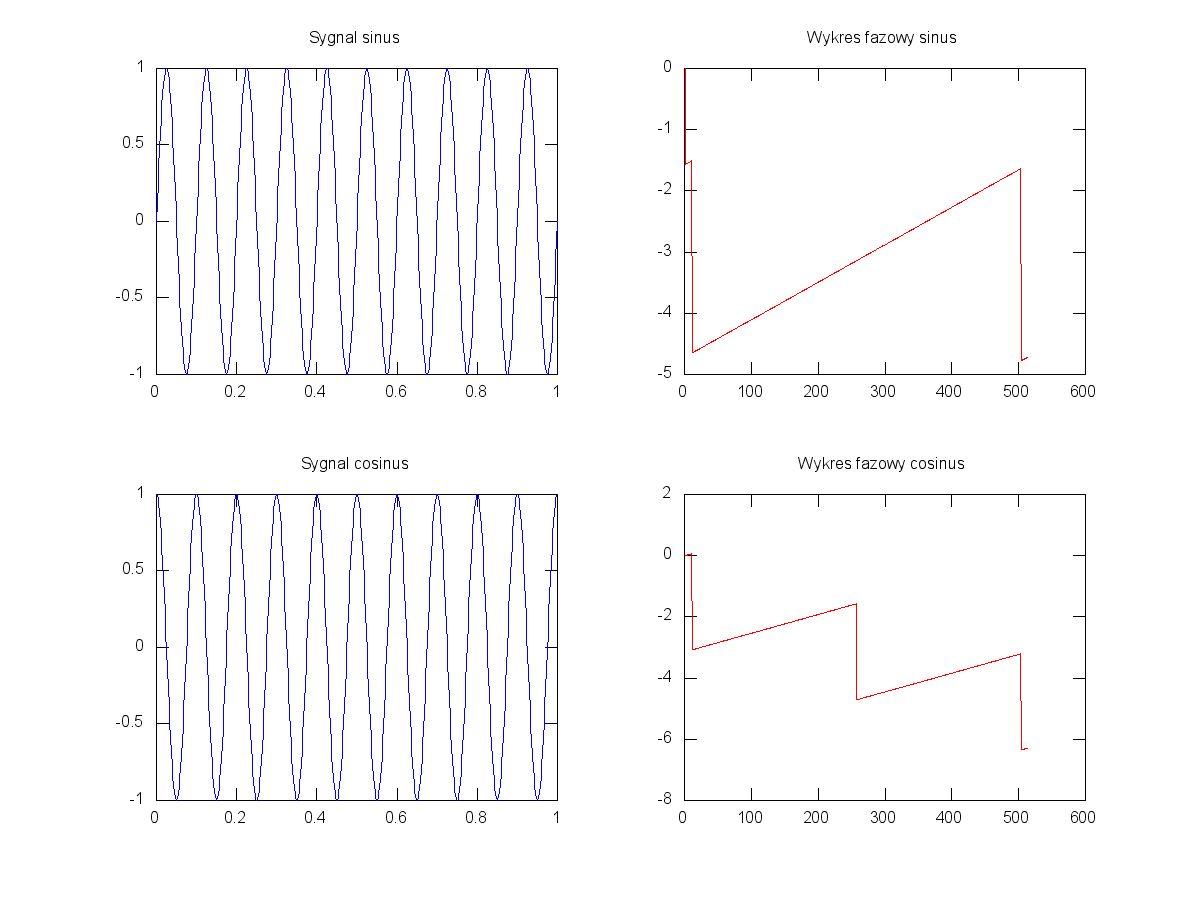
\includegraphics[scale=.5]{out/fig5.png}
	      \caption{\label{fig5} Wykresy fazowe sinus i cosinus}
	    \end{center}
	  \end{figure}
	\end{landscape}
	
	\begin{landscape}
	  \begin{figure}[htbp]
	    \begin{center}
	      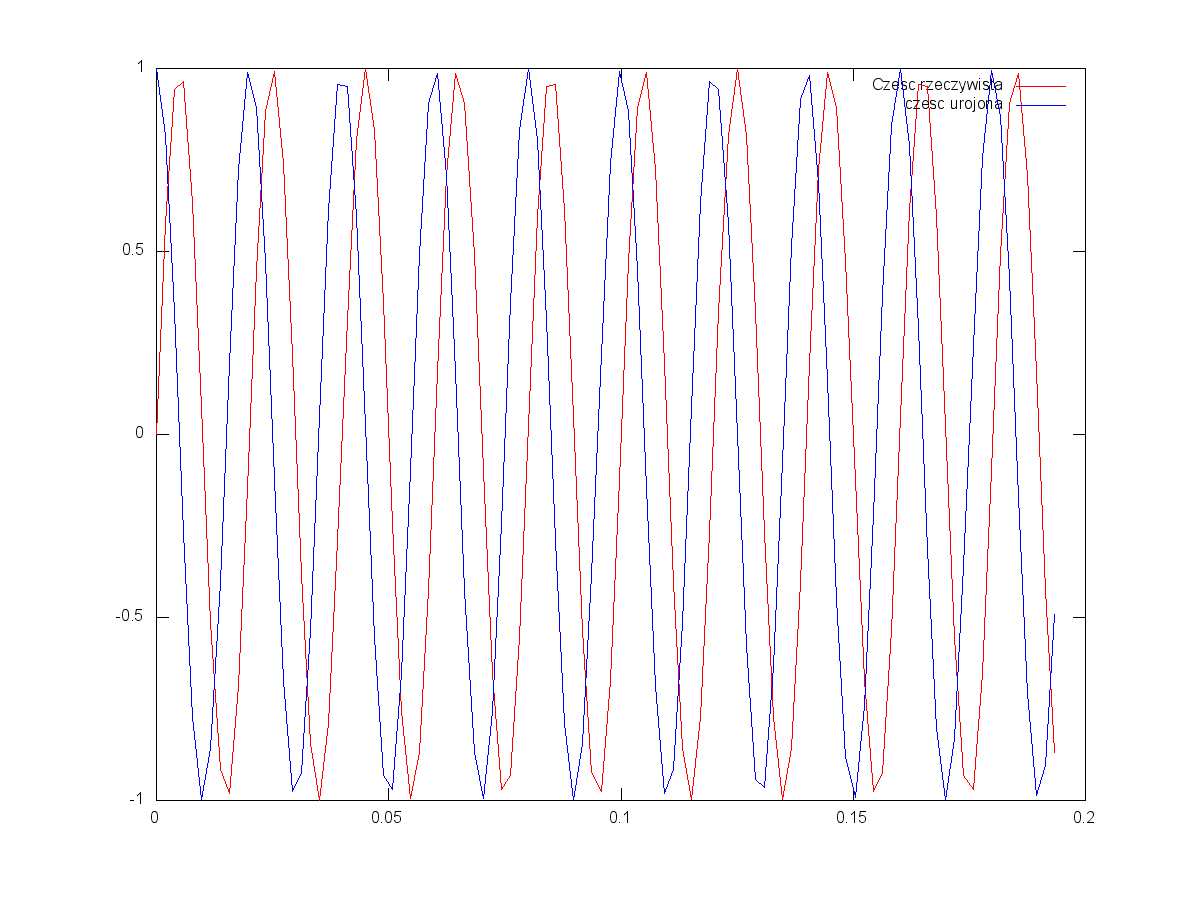
\includegraphics[scale=.5]{out/fig6.png}
	      \caption{\label{fig6} Sygnał zespolony, część rzeczywista i urojona}
	    \end{center}
	  \end{figure}
	\end{landscape}
	
	\begin{landscape}
	  \begin{figure}[htbp]
	    \begin{center}
	      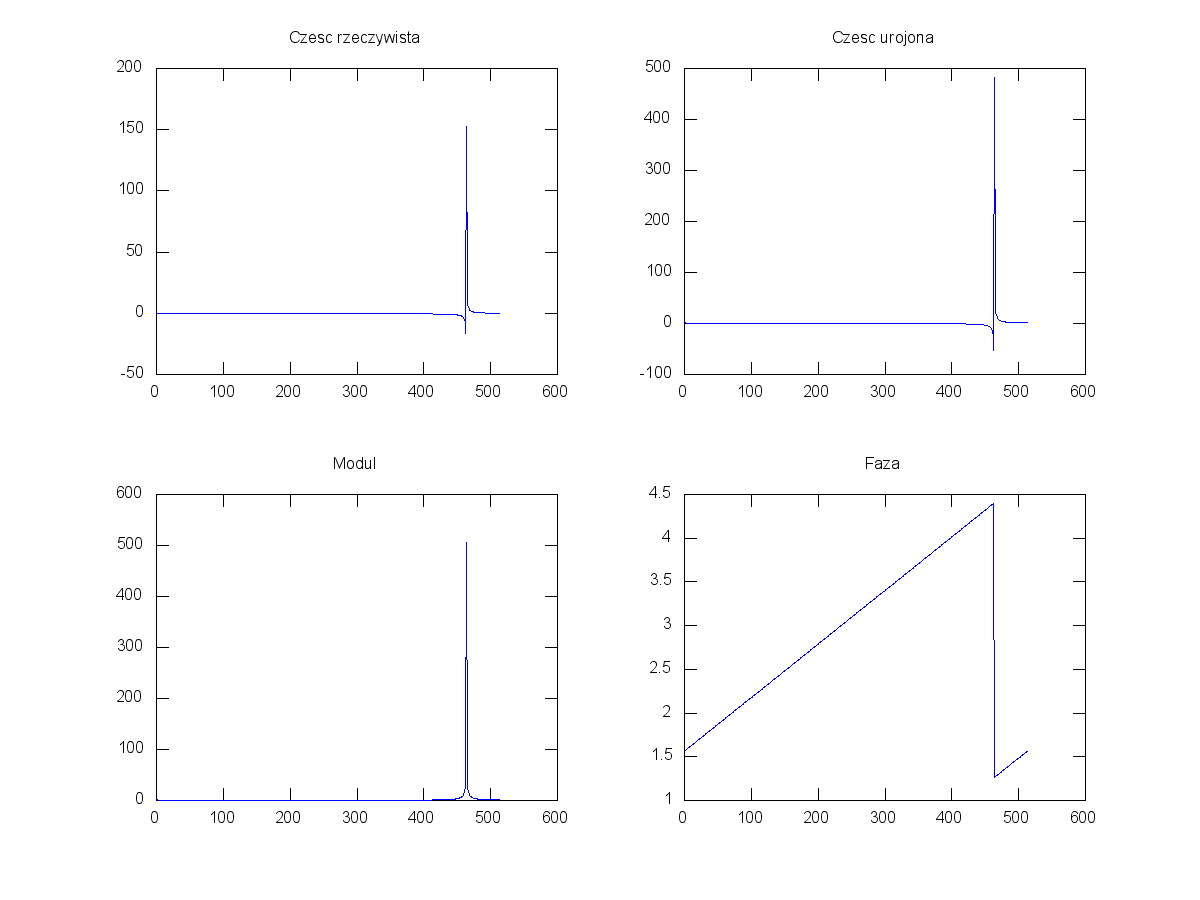
\includegraphics[scale=.5]{out/fig7.png}
	      \caption{\label{fig7} Widmo sygnału zespolonego}
	    \end{center}
	  \end{figure}
	\end{landscape}


\end{document}